{\tikzstyle{level 1}=[sibling distance=6\baselineskip, level distance=0.5cm]
\tikzstyle{level 2}=[sibling distance=6\baselineskip, level distance=0.5cm]
\centerline{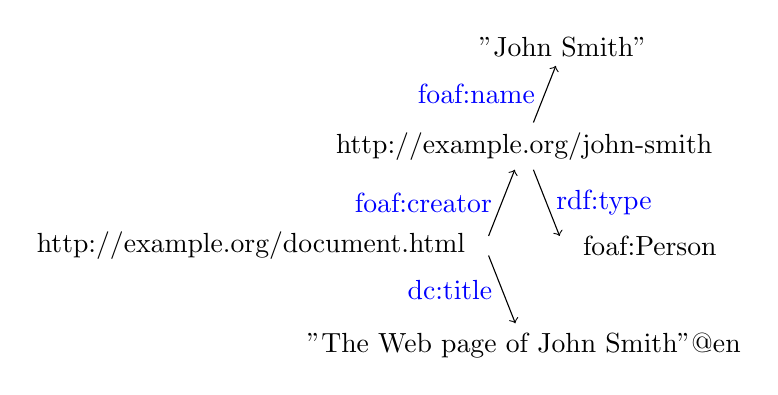
\begin{tikzpicture}[grow=right,->]
  \node[label=left:{\url{http://example.org/document.html}}] {}
    child { node {\code{"The Web page of John Smith"@en}}
      edge from parent
      node[left] {\textcolor{blue}{dc:title}}}
    child { node {\url{http://example.org/john-smith}}
      child { node[label=right:{foaf:Person}] {}
        edge from parent
        node[right,align=left] {\textcolor{blue}{rdf:type}}}
      child { node {\code{"John Smith"}}
        edge from parent
        node[left] {\textcolor{blue}{foaf:name}}}
      edge from parent
      node[left] {\textcolor{blue}{foaf:creator}};
    };
\end{tikzpicture}}}
